\section{Problema}
\subsection{Motivación}
\begin{frame}%\frametitle{Motivación}
    \begin{block}{Motivación}
    \begin{itemize} 
    	\item Los servicios de fibra al hogar \emph{(Fiber-To-The-Home - FTTH)} tienen una gran penetración mundial brindando a los clientes finales transferencias de datos a altas velocidades.
    	\item La cantidad de aplicaciones y servicios sobre internet ha crecido exponencialmente.
    	\item Es mandatorio escalar de forma inteligente la infraestructura de red.
    	\item Dado que el despligue de la fibra optica es una importante inversión económica, el diseño topológico de las redes \emph{FTTH} debe continuar considerandose.
	\end{itemize} 
    \end{block}
\end{frame}

\subsection{Objetivos I}
\begin{frame}
	\frametitle{}
    \begin{block}{Objetivos I}
	\begin{itemize} 
    	\item Problema de optimización combinatoria motivado por el diseño topológico de redes de comunicaciones 
con restricciones de confiabilidad.
		\item El objetivo es interconectar nodos distinguidos, llamados terminales, utilizando un nivel adecuado de redundancia y de forma simultanea, satisfacer las restricciones de confiabilidad.
	\item En el análisis de confiabilidad nos enfrentamos a fallas aleatorias en los componentes del sistema. Se considera el modelo como realista hostil, donde tanto nodos como aristas pueden fallar.
	\end{itemize} 
    \end{block}
\end{frame}

\subsection{Objetivos II}
\begin{frame}
	\frametitle{}
    \begin{block}{Objetivos II}
	\begin{itemize} 
    	\item Encontrar una solución de costo mínimo que alcance un umbral de confiabilidad, donde tanto los nodos como los enlaces pueden fallar con probabilidades dadas.
		\item Entender el trade-off entre costo-confiabilidad, y como la confiabilidad aumenta naturalmente agregando niveles de redundancia entre los nodos terminales.
		\item Entender el impacto en la confiabilidad de las redes solución al aumentar o disminuir las probabilidades de falla elementales tanto en nodos como enlaces.
    	\item Pertenece a la clase de problemas \emph{NP-Hard}.
    	\item Se propone una solución que resuelve el problema de forma apróximada con una metodología \emph{GRASP/VND} para el problema de optimización y para el análisis de la confiabilidad el método \emph{RVR}.
	\end{itemize} 
    \end{block}
\end{frame}

\subsection{Definición}
\begin{frame}\frametitle{Generalized Steiner Problem with Node-Connectivity Constraints and
Hostile Reliability GSPNCHR}
    \begin{definition}[GSPNCHR]
Se considera el grafo no dirigido $G=(V,E)$, conjunto de nodos terminales $T \subseteq V$, costo de los enlaces $\{c_{i,j}\}_{(i,j) \in E}$ y requerimientos de conectividad $R=\{r_{i,j}\}_{i,j \in T}$. Además, asumimos que tanto los enlaces como los nodos no terminales (Steiner) fallan con probabilidades $P_E=\{p_e\}_{e\in E}$ y $P_{V-T}=\{p_v\}_{v\in V-T}$. 
Dado el umbral de confiabilidad $p_{min}$, el objetivo es construir una topologia de costo mínimo $G_S \subseteq G$ cumpliendo con los requerimientos de conectividad $R$ y el umbral de confiabilidad: $R_{K}(G_S) \geq p_{min}$, siendo $K=T$ el conjunto de nodos terminales.
\end{definition}
\end{frame}

\subsection{Formulación como problema de programación matematica}
\begin{frame}\frametitle{GSPNCHR}
\begin{align}
\min &\sum_{(i,j)\in E} c_{i,j}x_{i,j} \notag \\
s.t. x_{ij}&\geq y_{(i,j)}^{u,v}+y_{(j,i)}^{u,v} \forall (i,j)\in E,
\forall u,v\in T, u \neq v \\
\sum_{(u,i)\in E}y_{(u,i)}^{u,v} &\geq r_{u,v} \, \, \forall \, u,v\in T, \, u\neq v \\
\sum_{(j,v)\in E}y_{(j,v)}^{u,v} &\geq r_{u,v} \, \, \forall \, u,v\in T, \, u\neq v \\
\sum_{(i,p)\in I(p)}y_{(i,p)}^{u,v}  - \sum_{(p,j)\in I(p)}y_{(p,j)}^{u,v}&\geq 0, \, \forall p\in V-\{u,v\}, \, \forall u,v\in T, \, u \neq v \notag \\
\end{align}
\end{frame}

\subsection{Formulación como problema de programación matematica}
\begin{frame}\frametitle{GSPNCHR}
\begin{align}
\sum_{(s,i)\in E} x_{s,i} &\leq M \hat{x}_{s}, \, \forall s\in V-T \\
R_{K}(G_S(\{x_{ij}\})) &\geq p_{min} \\
x_{(i,j)} &\in \{0,1\} \, \forall (i,j)\in E \\
\hat{x}_{i} &\in \{0,1\} \, \forall i \in V-T  \\
 y_{(i,j)}^{u,v} &\in \{0,1\} \, \forall (i,j)\in E, \, \forall u,v \in T, \, u \neq v
\end{align}
\end{frame}

\section{Resultados Teóricos}
\subsection{Resultados Teóricos}
\begin{frame}
	\frametitle{}
    \begin{block}{Resultados Teóricos}
    \begin{small}
		\begin{itemize} 
    		\item Se demuestra la complejidad computacional del problema \emph{(NP-hardness)}.
			\item Se modela el problema para instancias particulares con $r_{ij} = k, k \geq 2$, tanto para nodo conectividad como para enlace conectividad.
			\item Se encuentran cotas inferiores para las formulaciones anteriores aplicando teoría de dualidad y relajación lagrangiana.
	    	\item Formulación de programación matemática del problema para las versiones $k$ nodo-conectividad y $k$ arista-conectividad aplicando los teoremas de BienStock y Monma.
    		\item Se proponen algoritmos de orden polinomial para la resolución del problema en forma exacta de casos particulares respecto a conectividad y topología de grafos.
    	\end{itemize} 
    			\end{small}
    \end{block}
\end{frame}

\section{Estado del arte}
\subsection{Trabajos Relacionados}
\begin{frame}\frametitle{}
\begin{block}{Trabajos Relacionados}
	\begin{itemize} 
    	\item Se dedicó un capítulo entero donde se expone el relevamiento del estado del arte de la temática de esta tesis: Confiabilidad en redes, Diseño topológico de redes, GRASP, VND, RVR y otras como Monte Carlo Crudo.
    	\item Son escasos los trabajos que abordan conjuntamente la optimización topológica de la red  bajo restricciones de confiabilidad.
    	\item VND y RVR han sido utilizados con gran éxito en problemas de optimización combinatoria.
    \end{itemize} 
\end{block}
\end{frame}

\subsection{Publicación}
\begin{frame}\frametitle{}
\begin{block}{Publicación}
	\begin{enumerate}
		\begin{small}
			\item A GRASP/VND Heuristic for the Generalized Steiner Problem with Node-Connectivity Constraints and Hostile Reliability to be published in the Proceedings of the 8th International Conference on Variable Neighborhood Search (ICVNS March 2021). Khalifa University, Abu Dhabi, U.A.E. The article will be published by Springer in the Lecture Notes in Computer Science (LNCS) series.	
		\end{small}
	\end{enumerate}
\end{block}
\end{frame}

\section{Solución}
\subsection{Metodología}
\begin{frame}\frametitle{GRASP/VND}
\begin{block}{}
\begin{small}
\begin{itemize}
 \item Utilizamos una metodología GRASP/VND.
 \item GRASP y VND son metaheurísticas bien conocidas que se han utilizado con éxito para resolver muchos problemas difíciles de optimización combinatoria.
 \item GRASP es un poderoso proceso de arranque múltiple que opera en dos fases. Se construye una solución factible en una primera fase, cuyo vecindario luego se explora en la fase de búsqueda local.
 \item VND explora varias estructuras de vecindad en un orden determinista. Su éxito se basa en el simple hecho de que las diferentes estructuras de vecindad no suelen tener el mismo mínimo local. Así, la solución resultante es simultáneamente una solución localmente óptima en todas las estructuras vecinas.
\end{itemize} 
\end{small}
\end{block}
\end{frame}

\subsection{Esquema General}
\begin{frame}\frametitle{}
    \begin{block}{Network Design}
\begin{algorithm}[H]
\floatname{algorithm}{Alg}
\caption{$sol = NetworkDesign(G_B,iter,k,p_{min},P_E,P_{V-T},simiter)$}
\begin{algorithmic}[1]
\begin{small}    
\STATE $i \leftarrow 0; \, P \leftarrow \emptyset; \, sol \leftarrow \emptyset$
\WHILE {$i < iter$}
\STATE $\overline{g} \leftarrow Construction(G_B,P,k)$
\STATE $g_{sol} \leftarrow VND(\overline{g},P)$
\STATE $reliability \leftarrow RVR(g_{sol},P_E,P_{V-T},simiter)$
\IF{$reliability > p_{min}$}
\STATE $sol \leftarrow sol \cup \{g_{sol}\}$
\ENDIF
\ENDWHILE
\RETURN $sol$
\end{small}
\end{algorithmic}
\end{algorithm}
    \end{block}
\end{frame}

\subsection{GRASP - Fase Construcción}
\begin{frame}\frametitle{}
    \begin{block}{}
\begin{algorithm}[H]
\floatname{algorithm}{Alg}
\caption{$(sol,P) = Construction(G_B,C,R,k)$}
\begin{algorithmic}[1]
\begin{scriptsize}
\STATE $g_{sol} \leftarrow (S_D^{(I)},\emptyset)$; $m_{i,j}\leftarrow r_{i,j}$; $P_{i,j}\leftarrow \emptyset, \forall i,j \in S_{D}^{(I)}$; $A_{i,j}\leftarrow 0, \forall i,j \in S_{D}^{(I)}$
\WHILE {$\exists \, m_{i,j}>0: A_{i,j}<MAXATTEMPTS$}
\STATE $(i,j) \leftarrow ChooseRandom(S_{D}^{(I)}: m_{i,j}>0)$
\STATE $\overline{G} \leftarrow G_B \setminus P_{i,j}$
\FORALL {$(u,v)\in E(\overline{G})$}
\STATE $\overline{c}_{u,v} \leftarrow c_{u,v} \times 1_{\{(u,v) \notin g_{sol}\}}$
\ENDFOR
\STATE $L_p \leftarrow KSP(k,i,j,\overline{G},\overline{C})$
\IF{$L_p=\emptyset$}
\STATE $A_{i,j} \leftarrow A_{i,j}+1$; $P_{i,j} \leftarrow \emptyset$; $m_{i,j}\leftarrow r_{i,j}$ 
\ELSE 
\STATE $p \leftarrow SelectRandom(L_p)$; $g_{sol} \leftarrow g_{sol} \cup \{p\}$
\STATE $P_{i,j} \leftarrow P_{i,j} \cup \{p\}$; $m_{i,j} \leftarrow m_{i,j}-1$
\STATE $(P,M) \leftarrow GeneralUpdateMatrix(g_{sol},P,M,p,i,j)$
\ENDIF
\ENDWHILE
\RETURN $(g_{sol},P)$
\end{scriptsize}    
\end{algorithmic}
\end{algorithm}
\end{block}
\end{frame}

\subsection{Fase Búsqueda Local}
\begin{frame}\frametitle{}
\begin{block}{VND}
\begin{small}
El objetivo es combinar una rica diversidad de vecindades para obtener una solución óptima local para cada vecindario. NetworkDesign considera una implementación clásica de VND, ordenando las respectivas búsquedas locales después de la fase de construcción. Se consideran tres estructuras de vecindad para construir VND.
\begin{enumerate}
 \item SwapKeyPathLocalSearch
 \item KeyPathLocalSearch
 \item KeyTreeLocalSearch
\end{enumerate} 
\end{small}
\end{block}
\end{frame}

\subsection{Definiciones}
\begin{frame}\frametitle{}
\begin{definition}[key-node]
Un key-node $v$ en una solución factible $v \in g_{sol}$ es un nodo de Steiner (no terminal) con grado mayor o igual a tres.
\end{definition}
\begin{definition}[key-path]
Un key-path $p$ en una solución factible $p \subseteq g_{sol}$ es un camino elemental 
donde todos los nodos intermedios no son terminales con grado dos en $g_{sol}$, 
y los nodos extremos son terminales o key-nodes.
\end{definition}
\begin{definition}[key-tree]
Sea $v \in g_{sol}$ un key-node perteneciente a una solución factible $g_{sol}$. 
El key-tree asociado a $v$, denotado como $T_v$, es un árbol compuesto por todos los 
key-paths que se encuentran en un punto común (i.e., el key-node $v$).
\end{definition}
\end{frame}

\subsection{SwapKeyPathLocalSearch}
\begin{frame}\frametitle{}
\begin{small}
\begin{definition}[Estructura de Vecindad para Swap Key-Paths]
Dado un key-path $p \subseteq g_{sol}$, una solución vecina para $g_{sol}$ es 
$\hat{g}_{sol} = \{ g_{sol}\setminus p \}\cup \{m\}$, 
siendo $m$ el conjunto de nodos y enlaces que serán añadidos preservando la factibilidad de ${\hat{g}}_{sol}$.  
\end{definition}
\end{small}
\begin{block}{}
\begin{algorithm}[H]
\floatname{algorithm}{Alg}
\caption{$g_{sol} = SwapKeyPathLocalSearch(G_B,C,g_{sol},P)$}
\begin{algorithmic}[1]
\begin{scriptsize}
\STATE $improve \leftarrow TRUE$
\WHILE {$improve$}
\STATE $improve \leftarrow FALSE$
\STATE $K(g_{sol}) \leftarrow \{p_1,\ldots,p_h\}$ /* Key-path decomposition of $g_{sol}$ */
\WHILE{\textbf{not} $improve$ \textbf{and} $\exists$ \textbf{key-paths not analyzed}}
\STATE $p \leftarrow(K(g_{sol}))$ /* Path not analyzed yet */
\STATE $(g_{sol},improve) \leftarrow FindSubstituteKeyPath(g_{sol},p,P)$
\ENDWHILE
\ENDWHILE
\RETURN $g_{sol}$
\end{scriptsize}
\end{algorithmic}
\end{algorithm}
\end{block}
\end{frame}

\subsection{KeyPathLocalSearch}
\begin{frame}\frametitle{}
\begin{definition}[Estructura de Vecindad para Key-Paths]
\begin{tiny}
Dado un key-path $p \in g_{sol}$, una solución vecina es 
${\hat{g}}_{sol} = \{g_{sol} \setminus p \} \cup \{\hat{p}\}$, 
donde $\hat{p}$ es otro camino que conecta los extremos desde $p$.  
La vecindad de key-paths desde $g_{sol}$ esta compuesta por la operación previa 
a los posibles miembros pertenecientes a $K_{g_{sol}}$. 
\end{tiny}
\end{definition}
\begin{block}{}
\begin{algorithm}[H]
\floatname{algorithm}{Alg}
\caption{$g_{sol} = KeyPathLocalSearch(G_B,C,g_{sol})$}
\begin{algorithmic}[1]
\begin{tiny}
\STATE $improve \leftarrow TRUE$
\WHILE {$improve$}
\STATE $improve \leftarrow FALSE$
\STATE $K(g_{sol}) \leftarrow \{p_1,\ldots,p_h\}$ /* Key-path decomposition of $g_{sol}$ */
%\COMMENT{Key-path decomposition of $g_{sol}$}
\WHILE{\textbf{not} $improve$ \textbf{and} $\exists$ \textbf{key-paths not analyzed}}
\STATE $p \leftarrow(K(g_{sol}))$ /* Path not analyzed yet, with extremes $u$ and $v$ */
\STATE $\hat{\mu} \leftarrow <NODES(p) \cup S_D\setminus NODES(g_{sol}) > $ /* Induced subgraph $\hat{\mu}$ */
\STATE $\hat{p} \leftarrow Dijkstra(u,v,\hat{\mu})$
\IF{$COST(\hat{p}) < COST(p)$}
\STATE $g_{sol} \leftarrow \{ g_{sol}\setminus p \} \cup \{\hat{p}\}$
\STATE $improve \leftarrow TRUE$
\ENDIF
\ENDWHILE
\ENDWHILE
\RETURN $g_{sol}$
\end{tiny}
\end{algorithmic}
\end{algorithm}
\end{block}
\end{frame}

\subsection{KeyTreeLocalSearch}
\begin{frame}\frametitle{}
\begin{definition}[Estructura de Vecindad para Key-Tree]
\begin{small}
Se considera el key-tree $T_v \in g_{sol}$ con raíz key-node $v$.  
Un vecino de $g_{sol}$ es $\hat{g}_{sol} = \{ g_{sol}\setminus T_v \} \cup \{T\}$, siendo 
$T$ otro árbol que reemplaza a $T_v$ con hojas identicas. 
\end{small}
\end{definition}
\begin{block}{}
\begin{algorithm}[H]
\floatname{algorithm}{Alg}
\caption{$g_{sol} = KeyTreeLocalSearch(G_B,C,g_{sol})$}
\begin{algorithmic}[1]
\begin{scriptsize}
\STATE $improve \leftarrow TRUE$
\WHILE {$improve$}
\STATE $improve \leftarrow FALSE$
\STATE $ X \leftarrow KeyNodes(g_{sol})$ /* Key-nodes from $g_{sol}$ */
\STATE $\overline{S} \leftarrow S_D \setminus NODES(g_{sol})$
\WHILE{\textbf{not} $improve$ \textbf{and} $\exists$ \textbf{key-nodes not analyzed}}
\STATE $v \leftarrow X$ /* Key-node not analyzed yet */
\STATE $[g_{sol},improve] \leftarrow GeneralRecConnect(G_B,C,g_{sol},v,\overline{S})$
\ENDWHILE
\ENDWHILE
\RETURN $g_{sol}$
\end{scriptsize}
\end{algorithmic}
\end{algorithm}
\end{block}
\end{frame}

\subsection{Confiabilidad}
\begin{frame}\frametitle{}
\begin{block}{RVR}
\begin{scriptsize}
\begin{itemize}
 \item Metodo Recursivo de Reducción de Varianza.
 \item Objetivo reducir la red original en varias redes mas pequeñas de forma recursiva.
 \item Construir estimador de confiabilidad insesgado con menos varianza que Monte Carlo Crudo.
 %Sistema Binario Estocastico Monoto. 
\end{itemize} 
\end{scriptsize}
\end{block}
\begin{block}{}
\begin{algorithm}[H]
\floatname{algorithm}{Alg}
\caption{$RVR(G,K,p_v,p_e)$}
\begin{algorithmic}[1]
\begin{tiny}
\STATE \textbf{If} $terminals$=1, \textbf{return} $0$
\STATE \textbf{Elseif} $\phi(G,K)=1$, \textbf{return} 1.
\STATE \textbf{Else} 
\STATE $D := GetKExtendedCut(G)$
\STATE $Q_{D} := AllFailedProb(D)$
\STATE $index := GetRandomItem(D)$
\STATE $c := D[index]$
\STATE $remove(G,D, index - 1)$
\STATE $add(G, c)$
\STATE $return \, \, Q_{D} + (1 - Q_{D})\times RVR(G)$
\STATE \textbf{EndIf}
\end{tiny}
\end{algorithmic}
\end{algorithm}
\end{block}
\end{frame}

\section{Resultados}
\subsection{Resultados}
\begin{frame}\frametitle{}
\begin{block}{Conjunto de Casos de Prueba}
\begin{small}
\begin{itemize}
 \item Se realizó un extenso estudio computacional utilizando el algoritmo $NetworkDesign$.
 \item Adaptamos instancias conocidas de la librería $TSPLIB$ añadiendo probabilidades de falla en nodos y enlaces y los requerimientos de conectividad entre nodos.
  \item No hay casos benchmark para nuestro problema específico.
 \item Umbral de confiabilidad $p_{min}=0.8$.
 \item Probabilidades de nodos y aristas $p_v=0.99$ y $p_e=0.95$ respectivamente.
 \item Número de iteraciones en $NetworkDesign$ por cada instancia $iter=100$, y número de replicaciones para el método $RVR$ $10^4$.
 \item Comprender la sensibilidad de la solución a perturbaciones en confiabilidades elementales. Se utilizaron nueve combinaciones para $p_{v},p_{e} \in \{0.99, 0.97,0.95\}$.
\end{itemize} 
\end{small}
\end{block}
\end{frame}

\subsection{Resultados II}
\begin{frame}\frametitle{}
\begin{table}
\begin{scriptsize}
\caption{Conjunto de Casos de Prueba}
\end{scriptsize}
\centering
\scalebox{0.7}{
\begin{tabular}{|c|c|c|c|c|c|c|c|} % centered columns 
\hline	$Problem$   &	\% $T$ & \%$Rel$& \% $Req$ & $Iter\_ND$ & $Iter\_RVR$ & \# \\
\hline	att48	&	20-35-50	&	99-95	&	100-0-0	&	100-100-100	&	$10^4$	&	3	\\
\hline	berlin52	&	20-35-50	&	99-95	&	100-0-0	&	100-100-100	&	$10^4$	&	3	\\
\hline	brazil58	&	20-35-50	&	99-95	&	100-0-0	&	100-100-100	&	$10^4$	&	3	\\
\hline	ch150	&	20-35-50	&	99-95	&	100-0-0	&	100-100-100	&	$10^4$	&	3	\\
\hline	d198	&	20-35-50	&	99-95	&	100-0-0	&	20-20-20	&	NA	&	3	\\
\hline	eil51	&	20-35-50	&	99-95	&	100-0-0	&	100-100-100	&	$10^4$	&	3	\\
%\hline	gr137	&	20-35-50	&	99-95	&	100-0-0	&	100-20-20	&	NA	&	3	\\
\hline	gr202	&	20-35-50	&	99-95	&	100-0-0	&	100-100-100	&	$10^4$	&	3	\\
\hline	kroA100	&	20-35-50	&	99-95	&	100-0-0	&	100-100-100	&	NA	&	3	\\
%\hline	kroA150	&	20-35-50	&	99-95	&	100-0-0	&	100-20-20	&	NA	&	3	\\
\hline	kroB100	&	20-35-50	&	99-95	&	100-0-0	&	100-100-100	&	NA	&	3	\\
\hline	kroB150	&	20-35-50	&	99-95	&	100-0-0	&	100-20-20	&	NA	&	3	\\
\hline	kroB200	&	20-35-50	&	99-95	&	100-0-0	&	20-20-20	&	NA	&	3	\\
\hline	lin105	&	20-35-50	&	99-95	&	100-0-0	&	100-100-100	&	NA	&	3	\\
\hline	pr152	&	20-35-50	&	99-95	&	100-0-0	&	20-20-20	&	NA	&	3	\\
%\hline	rat195	&	20-35-50	&	99-95	&	100-0-0	&	20-20-20	&	NA	&	3	\\
%\hline	st70	&	20-35-50	&	99-95	&	100-0-0	&	100-100-100	&	$10^4$	&	3	\\
\hline	tsp225	&	20-35-50	&	99-95	&	100-0-0	&	50-50-50	&	$10^4$	&	3	\\
%\hline	u159	&	20-35-50	&	99-95	&	100-0-0	&	20-20-20	&	NA	&	3	\\
%\hline	rd100	&	20-35-50	&	99-95	&	100-0-0	&	100-100-100	&	NA	&	3	\\
\hline	rd400	&	20-35-50	&	99-95	&	100-0-0	&	50-50-50	&	$10^4$	&	3	\\
\hline	berlin52(E)	&	20	&	99-90	&	65-25-10	&	100	&	$10^4$	&	1	\\
%\hline	eil51(E)	&	20	&	99-90	&	65-25-10	&	100	&	$10^4$	&	1	\\
\hline	att48(E)	&	35	&	99-90	&	65-25-10	&	100	&	$10^4$	&	1	\\
%\hline	st70(E)	&	35	&	99-90	&	65-25-10	&	100	&	$10^4$	&	1	\\
\hline	brazil58(E)	&	50	&	99-90	&	65-25-10	&	100	&	$10^4$	&	1	\\
%\hline	eil51(E)	&	50	&	99-90	&	65-25-10	&	100	&	$10^4$	&	1	\\
%\hline	kroB100(E)	&	20	&	99-90	&	65-25-10	&	100	&	$10^4$	&	1	\\
%\hline	lin105(E)	&	20	&	99-90	&	65-25-10	&	100	&	NA	&	1	\\
%\hline	kroA100(E)	&	35	&	99-90	&	65-25-10	&	20	&	$10^4$	&	1	\\
\hline	rd100(E)	&	35	&	99-90	&	65-25-10	&	20	&	NA	&	1	\\
\hline
\end{tabular}}
\end{table}
\end{frame}

\subsection{Resultados III}
\begin{frame}\frametitle{}
\begin{table}
\begin{scriptsize}
\caption{GRASP/VND Effectiveness}
\end{scriptsize}
\centering
\scalebox{0.7}{
\begin{tabular}{|c|c|c|c|c|c|c|} % centered columns 
\hline	$Problem$   &	\% $T$ & \%$IC$& \% $IVND$ & $CPU(s)$ & $\overline{R}$ & $\overline{Var}$ \\
\hline	att48	&	20	&	99.27	&	34.61	&	11.466	&	0.967	&	7.608E-07	\\
\hline	att48	&	35	&	98.6	&	36.83	&	29.769	&	0.943	&	3.448E-06	\\
\hline	att48	&	50	&	98.22	&	37.1	&	65.904	&	0.927	&	5.322E-06	\\
\hline	berlin52	&	20	&	98.98	&	30.55	&	30.605	&	0.937	&	3.294E-06	\\
\hline	berlin52	&	35	&	99.06	&	33.93	&	33.433	&	0.938	&	3.19E-06	\\
\hline	berlin52	&	50	&	98.02	&	33.48	&	106.945	&	0.907	&	6.487E-06	\\
\hline	brazil58	&	20	&	98.92	&	31.96	&	62.377	&	0.885	&	6.722E-06	\\
\hline	brazil58	&	35	&	99.25	&	39.45	&	68.891	&	0.86	&	8.347E-06	\\
\hline	brazil58	&	50	&	98.75	&	35.26	&	103.553	&	0.91	&	7.093E-06	\\
\hline	ch150	&	20	&	99.76	&	37.51	&	222.552	&	0.8559	&	1.029E-05	\\
\hline	ch150	&	35	&	99.72	&	36.65	&	546.652	&	0.8803	&	9.033E-05	\\
\hline	gr202	&	20	&	99.89	&	32.43	&	100.162	&	0.8231	&	1.224E-05	\\
\hline	gr202	&	35	&	99.75	&	34.56	&	200.698	&	0.8414	&	1.11E-05	\\
\hline	gr202	&	50	&	99.74	&	33.36	&	600.629	&	0.8303	&	1.279E-05	\\
\hline	rd400	&	20	&	99.94	&	35.84	&	88.214	&	0.8094	&	14.22E-05	\\
\hline	rd400	&	35	&	99.94	&	33.54	&	504.103	&	0.8537	&	11.89E-05	\\
\hline	rd400	&	50	&	99.93	&	33.16	&	980.701	&	0.8643	&	11.51E-05	\\
\hline Average     & 35    &   99.28   &  34.72   &    220.980 &  0.884 & 3.28E-05 \\
\hline
\end{tabular}}
\end{table}
\end{frame}

\subsection{Resultados IV}
\begin{frame} \frametitle{Preguntas Claves}
\begin{tiny}
\begin{block} {1}
 	 \begin{itemize}
 	 	\item ¿Cuántas redes factibles existen dado el modelo probabilístico completo $(p_{min}:0.98,P_E:0.99,P_{V-T}:0.99)$?
 	 	\item La cantidad de soluciones que cumplen con el umbral de confiabilidad es alta. Alcanza el 100\% en la mayoría de los casos.
 	 \end{itemize}  
 \end{block} 	   
 \begin{block} {2}
 	 \begin{itemize}
 	 	\item ¿Cuál es la sensibilidad del modelo con respecto a las confiabilidades elementales? ¿Es mejor aumentar la confiabilidad elemental de los enlaces, o la confiabilidad de los nodos Steiner, para cumplir con un umbral de confiabilidad exigente?
 	 	\item El modelo es más sensible a fallas de enlace que a fallas de nodo. Un aumento en la confiabilidad de los enlaces tiene un mejor impacto que un aumento correspondiente en la confiabilidad de los nodos.
 	 \end{itemize}  
 \end{block} 	
  \begin{block} {3}
 	 \begin{itemize}
 	 	\item ¿Cuántas redes sobreviven en promedio, para cualquier modelo probabilístico dado? Comprender la sensibilidad del modelo con respecto a los requisitos de conectividad $r_{i,j} \in \{2,3,4\}$?
 	 	\item Podemos apreciar que un aumento en los requisitos de conectividad de la red implica necesariamente un aumento correspondiente en el porcentaje de redes que cumplen con el umbral de confiabilidad, y viceversa.
 	 \end{itemize}  
 \end{block} 	
 \end{tiny}
\end{frame}

\subsection{Resultados V}
\begin{frame}\frametitle{}
\begin{table}
\begin{scriptsize}
\caption{Soluciones factibles con $R \geq 0.98$,  
$p_v=0.99$ fijo y confiabilidad de enlaces variable.}
\end{scriptsize}
\centering  % used for centering table
\scalebox{0.7}{
\begin{tabular}{|c|c|c|c|c|} % centered columns 
\hline	Instance  &	$p_e=0.99$ & 	$p_e=0.97$ & 	$p_e=0.95$\\
\hline	att48 T20	&	100	&	90	&	12	\\
\hline	att48 T35	&	100	&	53	&	0	\\
\hline	att48 T50	&	100	&	20	&	0	\\
\hline	berlin52 T20	&	100	&	41	&	0	\\
\hline	berlin52 T35	&	100	&	50	&	0	\\
\hline	berlin52 T50	&	100	&	1	&	0	\\
\hline	brazil58 T20	&	99	&	15	&	0	\\
\hline	brazil58 T35	&	97	&	0	&	0	\\
\hline	brazil58 T50	&	100	&	5	&	0	\\
\hline	ch150 T20	&	100	&	0	&	0	\\
\hline	ch150 T35	&	100	&	0	&	0	\\
\hline	ch150 T50	&	100	&	0	&	0	\\
\hline	gr202 T20	&	99	&	0	&	0	\\
\hline	gr202 T35	&	100	&	0	&	0	\\
\hline	gr202 T50	&	100	&	0	&	0	\\
\hline	rd400 T20	&	100	&	0	&	0	\\
\hline	rd400 T35	&	100	&	0	&	0	\\
\hline	rd400 T50	&	100	&	0	&	0	\\
\hline  Average     & 99.72    &   15.28   &  0.67 \\
\hline
\end{tabular}}
\end{table}
\end{frame}

\subsection{Resultados VI}
\begin{frame}\frametitle{}
\begin{table}
\begin{scriptsize}
\caption{Soluciones factibles con $R \geq 0.98$, $p_e=0.99$ fijo 
y confiabilidad de nodos variable.}
\end{scriptsize}
\centering  % used for centering table
\scalebox{0.7}{
\begin{tabular}{|c|c|c|c|c|} % centered columns 
\hline	Instance  &	$p_v=0.99$ & 	$p_v=0.97$ & 	$p_v=0.95$\\
\hline	att48 T20	&	100	&	100	&	99	\\
\hline	att48 T35	&	100	&	98	&	96	\\
\hline	att48 T50	&	100	&	100	&	99	\\
\hline	berlin52 T20	&	100	&	100	&	80	\\
\hline	berlin52 T35	&	100	&	99	&	93	\\
\hline	berlin52 T50	&	100	&	100	&	100	\\
\hline	brazil58 T20	&	99	&	59	&	41	\\
\hline	brazil58 T35	&	97	&	43	&	9	\\
\hline	brazil58 T50	&	100	&	99	&	81	\\
\hline	ch150 T20	&	100	&	60	&	20	\\
\hline	ch150 T35	&	100	&	98	&	76	\\
\hline	ch150 T50	&	100	&	100	&	97	\\
\hline	gr202 T20	&	99	&	80	&	30	\\
\hline	gr202 T35	&	100	&	69	&	16	\\
\hline	gr202 T50	&	100	&	100	&	76	\\
\hline	rd400 T20	&	100	&	16	&	2	\\
\hline	rd400 T35	&	100	&	98	&	80	\\
\hline	rd400 T50	&	100	&	100	&	100	\\
\hline  Average     &   99.72    &   84.39   &  66.39 \\
\hline
\end{tabular}}
\end{table}
\end{frame}

\subsection{Resultados VII}
\begin{frame}\frametitle{}
\begin{block}{Brazil58}
\begin{scriptsize}
\%20 de nodos terminales, confiabilidad elemental de nodos de Steiner \%99, confiabilidad de enlaces \%95 y \%100 2 caminos nodo-disjunto. Nodos terminales rojos no fallan, nodos de Steiner naranjas y grises.
\end{scriptsize}
\begin{center}
   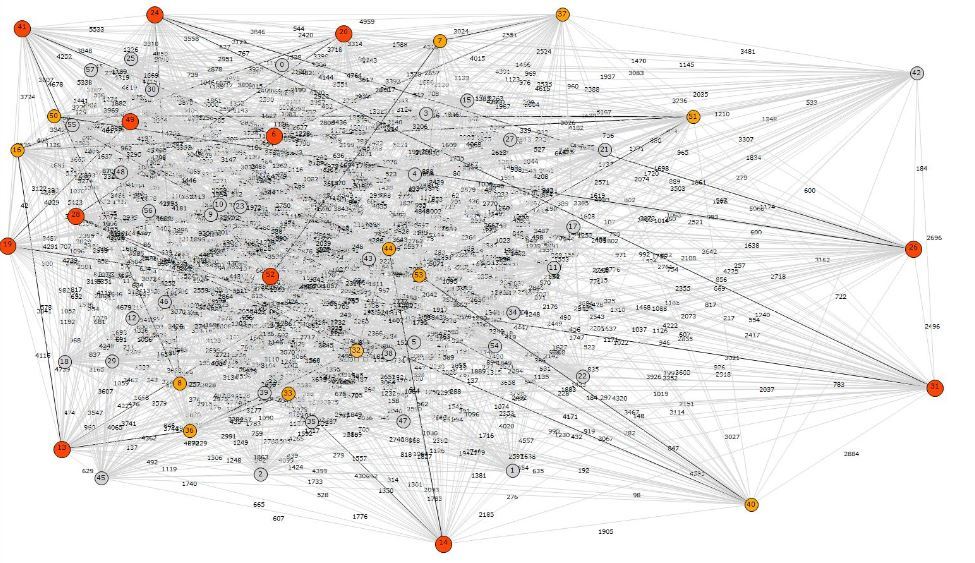
\includegraphics[scale=0.35]{figuras/1}
\end{center}
\end{block}
\end{frame}

\subsection{Resultados VIII}
\begin{frame}\frametitle{}
\begin{block}{Brazil58 NetworkDesign Salida}
\begin{scriptsize}
Costo resultado 25106 (32\% de mejora con respecto a la de construcción) y confiabilidad 92\%. 
\end{scriptsize}
\begin{center}
   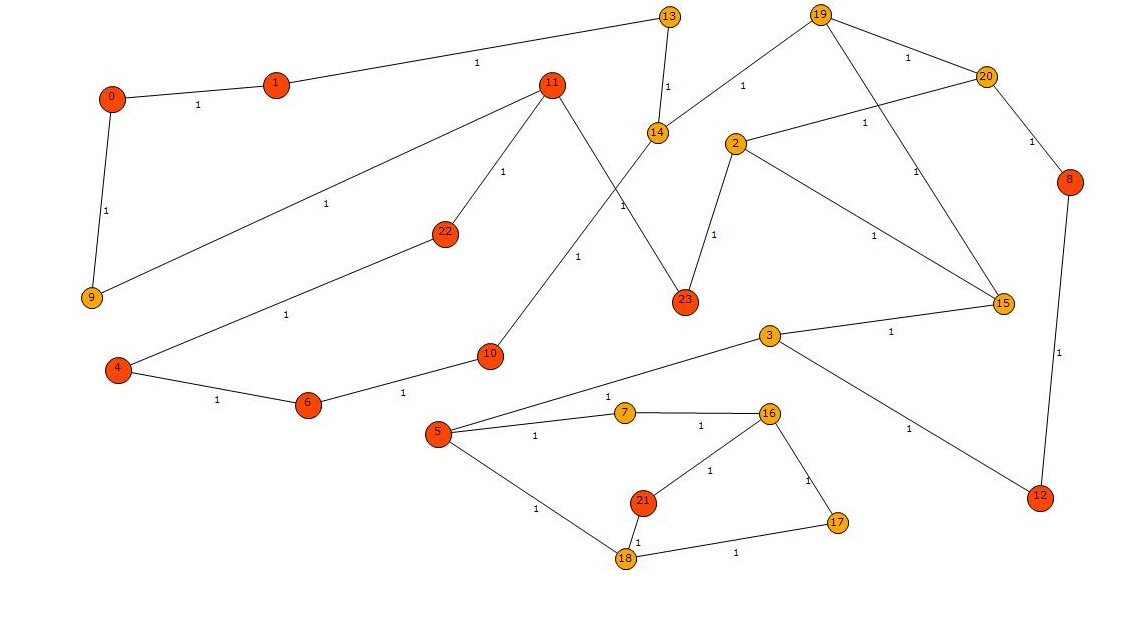
\includegraphics[scale=0.35]{figuras/2}
\end{center}
\end{block}
\end{frame}

\section{Conclusiones}
\subsection{Conclusiones}
\begin{frame} \frametitle{Conlusiones y Aportes de este Trabajo}
\begin{block} {}
   	\begin{itemize} 
   	\begin{scriptsize}
	\item Estudiamos el diseño topológico de redes de alta confiabilidad.
	\item Nuestro objetivo es combinar aspectos puramente deterministas como la conectividad con modelos probabilísticos provenientes de la confiabilidad de la red.
	\item Se introduce The Generalized Steiner Problem with Node-Connectivity Constraints and Hostile Reliability (GSPNCHR).
	\item Probamos formalmente que GSPNCHR pertenece a la clase NP-Hard.
	\item Como consecuencia se propone una metodología GRASP/VND.
	\end{scriptsize}   	     	
 	\end{itemize} 	
 \end{block}
\end{frame}

\subsection{Conclusiones II}
\begin{frame} \frametitle{Conlusiones y Aportes de este Trabajo}
\begin{block} {}
   	\begin{itemize} 
   	\begin{scriptsize}
	\item Dado que la evaluación de confiabilidad para el modelo hostil también pertenece a la clase NP-Hard, Adoptamos una excelente método de estimación de confiabilidad puntual, conocida como Recursive Variance Reduction (RVR).
	\item La mejora proporcionada por la fase VNS después de la fase de Construcción oscila entre el 25,25\% y el 39,84\%.
	\item La confiabilidad promedio para todas las redes varía entre 82.31\% y 99.87\%.
	\item Nuestros resultados resaltan que el modelo es más robusto bajo fallas en los nodos que bajo fallas en los enlaces.
	\item Se logró la publicación: A GRASP/VND Heuristic for the Generalized Steiner Problem with Node-Connectivity Constraints and Hostile Reliability, a publicarse en Volume 12559 of the Lecture Notes in Computer Science series.
	\end{scriptsize}   	     	
 	\end{itemize} 	
 \end{block}
\end{frame}

\subsection{Conclusiones III}
\begin{frame} \frametitle{Líneas de Trabajo Futuro}
\begin{block} {}
   	\begin{scriptsize}
 	 \begin{itemize}
 	 	\item La interacción entre el diseño de la red topológica y la confiabilidad de la red aún no se comprende bien. Aquí se propusieron algunas búsquedas locales, esencialmente utilizando reemplazos de key-path y key-tree, con el fin de reducir los costos y preservar la factibilidad.
 	 	\item Una línea de investigación actual es introducir transformaciones que aumenten la confiabilidad. 
 	 	\item El desarrollo de búsquedas locales que aumenten la confiabilidad y reduzcan los costos enriquecería la solución actual.
 	 	\item Otra posibilidad para el trabajo futuro es enriquecer el número de búsquedas locales y considerar transiciones probabilísticas entre ellas.
 	 	\item Mejorar en lo posible la algoritmia, apta para computación de alta performance y reducir los tiempos de cómputo.
 	 \end{itemize}  
 	\end{scriptsize}
 \end{block} 	   
\end{frame}

\subsection{Gracias}
\begin{frame} \frametitle{Fin}
\begin{huge}
Muchas Gracias.
\end{huge}
\end{frame}

\section{Anexos}
\subsection{Anexo}
\begin{frame}\frametitle{}
\begin{block}{Berlin52}
\begin{scriptsize}
\%20 de nodos terminales, confiabilidad elemental de nodos de Steiner \%99, confiabilidad de enlaces \%95 y \%100 2 caminos nodo-disjuntos.  Nodos terminales rojos no fallan, nodos de Steiner naranjas y grises.
\end{scriptsize}
\begin{center}
   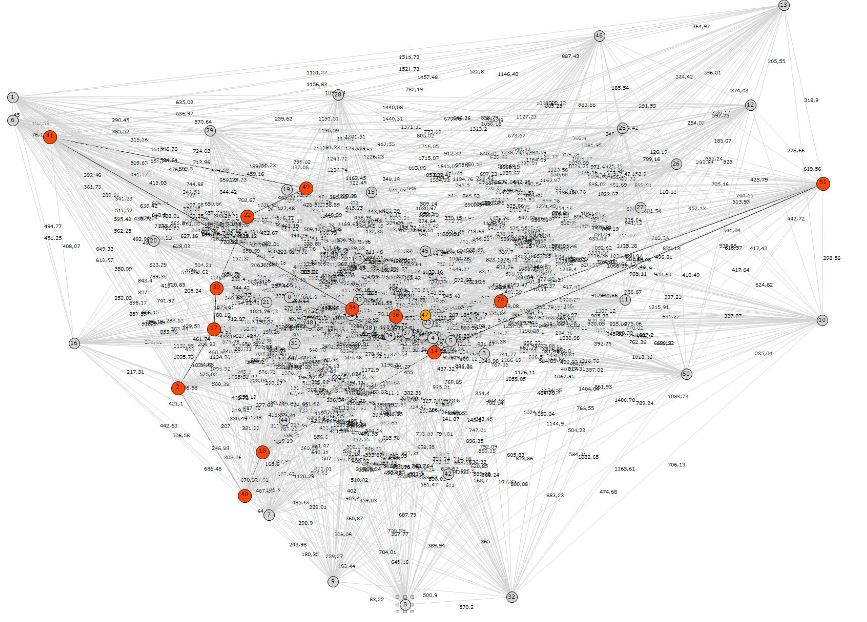
\includegraphics[scale=0.35]{figuras/3}
\end{center}
\end{block}
\end{frame}

\subsection{Anexo II}
\begin{frame}\frametitle{}
\begin{block}{Berlin52 Salida NetworkDesign}
\begin{scriptsize}
Costo resultado 4534 (31\% de mejora con respecto a la de construcción) y confiabilidad 84\%.
\end{scriptsize}
\begin{center}
   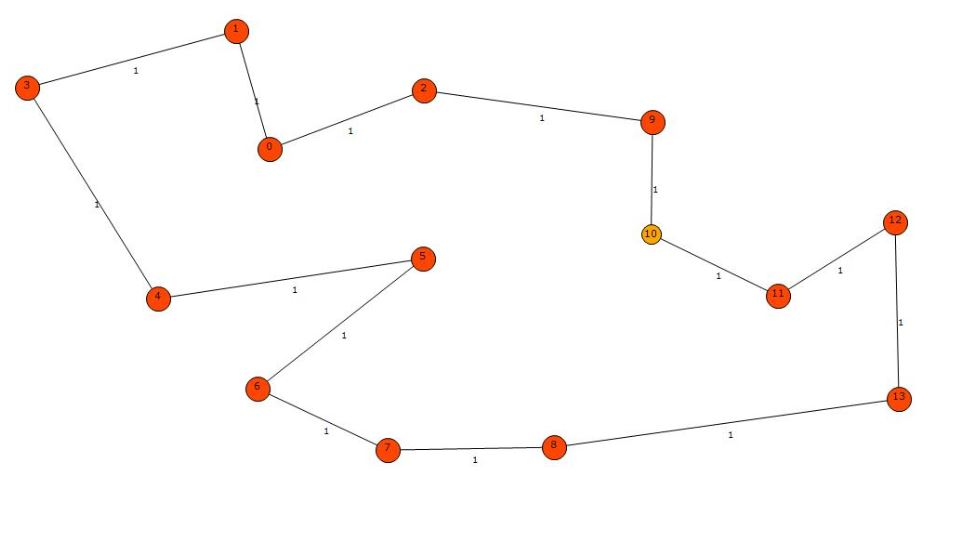
\includegraphics[scale=0.35]{figuras/4}
\end{center}
\end{block}
\end{frame}